\documentclass{beamer}

\mode<presentation> 
{
    % The Beamer class comes with a number of default slide themes
    % which change the colors and layouts of slides. Below this is a list
    % of all the themes, uncomment each in turn to see what they look like.

    \usetheme{default}
    %\usetheme{AnnArbor}
    %\usetheme{Antibes}
    %\usetheme{Bergen}
    %\usetheme{Berkeley}
    %\usetheme{Berlin}
    %\usetheme{Boadilla}
    %\usetheme{CambridgeUS}
    %\usetheme{Copenhagen}
    %\usetheme{Darmstadt}
    %\usetheme{Dresden}
    %\usetheme{Frankfurt}
    %\usetheme{Goettingen}
    %\usetheme{Hannover}
    %\usetheme{Ilmenau}
    %\usetheme{JuanLesPins}
    %\usetheme{Luebeck}
    %\usetheme{Madrid}
    %\usetheme{Malmoe}
    %\usetheme{Marburg}
    %\usetheme{Montpellier}
    %\usetheme{PaloAlto}
    %\usetheme{Pittsburgh}
    %\usetheme{Rochester}
    %\usetheme{Singapore}
    %\usetheme{Szeged}
    %\usetheme{Warsaw}

    % As well as themes, the Beamer class has a number of color themes
    % for any slide theme. Uncomment each of these in turn to see how it
    % changes the colors of your current slide theme.

    %\usecolortheme{albatross}
    %\usecolortheme{beaver}
    %\usecolortheme{beetle}
    %\usecolortheme{crane}
    %\usecolortheme{dolphin}
    %\usecolortheme{dove}
    %\usecolortheme{fly}
    %\usecolortheme{lily}
    %\usecolortheme{orchid}
    %\usecolortheme{rose}
    %\usecolortheme{seagull}
    %\usecolortheme{seahorse}
    %\usecolortheme{whale}
    %\usecolortheme{wolverine}

%\setbeamertemplate{footline} % To remove the footer line in all slides uncomment this line
%\setbeamertemplate{footline}[page number] % To replace the footer line in all slides with a simple slide count uncomment this line

%\setbeamertemplate{navigation symbols}{} % To remove the navigation symbols from the bottom of all slides uncomment this line
}

\usepackage{graphicx} % Allows including images
\usepackage{booktabs} % Allows the use of \toprule, \midrule and \bottomrule in tables
\usepackage{multirow}   % Allows including tables

\usepackage{beamerthemeshadow}
\usepackage{latexsym,amsbsy,amsopn,amstext,xcolor,multicol,amsmath}
\usepackage{amssymb,graphicx,wrapfig,fancybox}
\usepackage{pgf,pgfarrows,pgfnodes,pgfautomata,pgfheaps,pgfshade}
\usepackage{booktabs}
\usepackage{subfloat}
%\usepackage{multirow}
\usepackage{}
\graphicspath{{figures/}}

%----------------------------------------------------------------------------------------
%	TITLE PAGE
%----------------------------------------------------------------------------------------

\title[Group Report]{Group Report on Recent Work}

\author{Ma Hsuning}
\institute[NKU]
{
    Physics of NKU\\
    \medskip
    \textit{maxn@ihep.ac.cn}
}
\date{\today}

%----------------------------------------------------------------------------------------
\begin{document}
%----------------------------------------------------------------------------------------
\frame{\titlepage}
%----------------------------------------------------------------------------------------

\section{Recent work}
%----------------------------------------------------------------------------------------
\begin{frame}{Introduction to recent work}
\begin{itemize}
\item Input-output check upon the branching ratio of ${\eta}_c \rightarrow K_S K \pi$.
\bigskip
\item Observation of the signals of ${\eta}_c$ and $h_c$.
\end{itemize}
\end{frame}
%----------------------------------------------------------------------------------------

\section{Input-output check}
\begin{frame}{Input-output check}
We generated 200K MC sample of the decay\\
        \begin{center}
$\psi(3686)  \rightarrow {\pi}^0 h_c$,\\
        $h_c  \rightarrow \gamma {\eta}_c$,\\
        ${\eta}_c  \rightarrow K_S K \pi$.
        \end{center}
And we generated 200K MC sample of the decay\\
        \begin{center}
$\psi(3686)  \rightarrow {\pi}^0 h_c$,\\
        $h_c  \rightarrow \gamma {\eta}_c$,\\
        ${\eta}_c  \rightarrow \{anything\}$.
        \end{center}
\end{frame}
%----------------------------------------------------------------------------------------

\begin{frame}{Input-output check results}
\begin{table}
\begin{tabular}{|c|c|c|c|c|}
\hline
\hline
\multirow{2}{*}{Decay channel} & \multicolumn{2}{|c|}{\begin{tabular}{|c|}{Reconstruction\\ via $K_S$, $K$ and $\pi$}\end{tabular}} & \multicolumn{2}{|c|}{\begin{tabular}{|c|}{Recoil\\ via $\gamma$ and ${\pi}^0$}\end{tabular}}\\
\cline{2-5}
& $N_{obs}$ & $N_{tot}$ & $N_{obs}$ & $N_{tot}$\\
        \hline
${\eta}_c \rightarrow K_S K \pi$ & 27646 & 200K & 43412 & 200K\\
        \hline
${\eta}_c \rightarrow \{anything\}$ & 599 & 200K & 75686 & 200K\\
        \hline
\hline
\end{tabular}
\caption{Input-output check results}
\end{table}
Analysis is on the following page.
\end{frame}
%----------------------------------------------------------------------------------------

\begin{frame}{Input-output check results analysis and existing problems}
From the table on previous page, we can see that:
    \bigskip
\begin{itemize}
\item With reconstruction via $K_S$, $K$ and $\pi$, we have\\
        \begin{center}
        $Br({\eta}_c \rightarrow K_S K \pi) & =\frac{N_{obs}({\eta}_c\rightarrow \{anything\}) \times N_{tot}({eta}_c \rightarrow K_S K \pi)}{N_{tot}({\eta}_c\rightarrow \{anything\}) \times N_{obs}({eta}_c \rightarrow K_S K \pi)} \\
                \bigskip
        & =599/27646\\
                &= 0.02167$,\\
                \end{center}
which corresponds the branching ratio we used in the MC-generating, which is 0.0288.
\bigskip
\item With recoil via $\gamma$ and ${\pi}^0$, we don't under stand the reason why $N_{obs}({eta}_c \rightarrow K_S K \pi)$ and $N_{obs}({eta}_c \rightarrow \{anything\})$ are on the same level yet \large{\testbf{\color{red}different}}.
\end{itemize}
\end{frame}
%----------------------------------------------------------------------------------------

\section{Observation of the signals of $h_c$ and ${\etac}_c$}
\begin{frame}{Optimized selection}
We used the following optimized selections:
        \begin{itemize}
        \item $0<\chi_{1C}^2<5$;
        \item $0.11<m_{inv}^{\gamma \gamma}<0.145$;
        \item $0.46<E(\gamma_{E1})<0.53$;
        \item $|m_{recoil}(\pi^0 \pi^0)-M_{J/\psi}|<0.06$;
        \item $|m_{recoil}(\gamma)-M_{\chi_{c0}}|<0$;
        \item $|m_{recoil}(\gamma)-M_{\chi_{c1}}|<0.013$;
        \item $|m_{recoil}(\gamma)-M_{\chi_{c2}}|<0.0$;
        \item $|m_{recoil}(\pi^+ \pi^-)-M_{J/\psi}|<0.009$.
        \end{itemize}
\end{frame}
%----------------------------------------------------------------------------------------

        \begin{frame}{Distribution of recoil mass of $\gamma$ and $\pi^0$}
        \begin{center}
        \vskip -1.0cm
        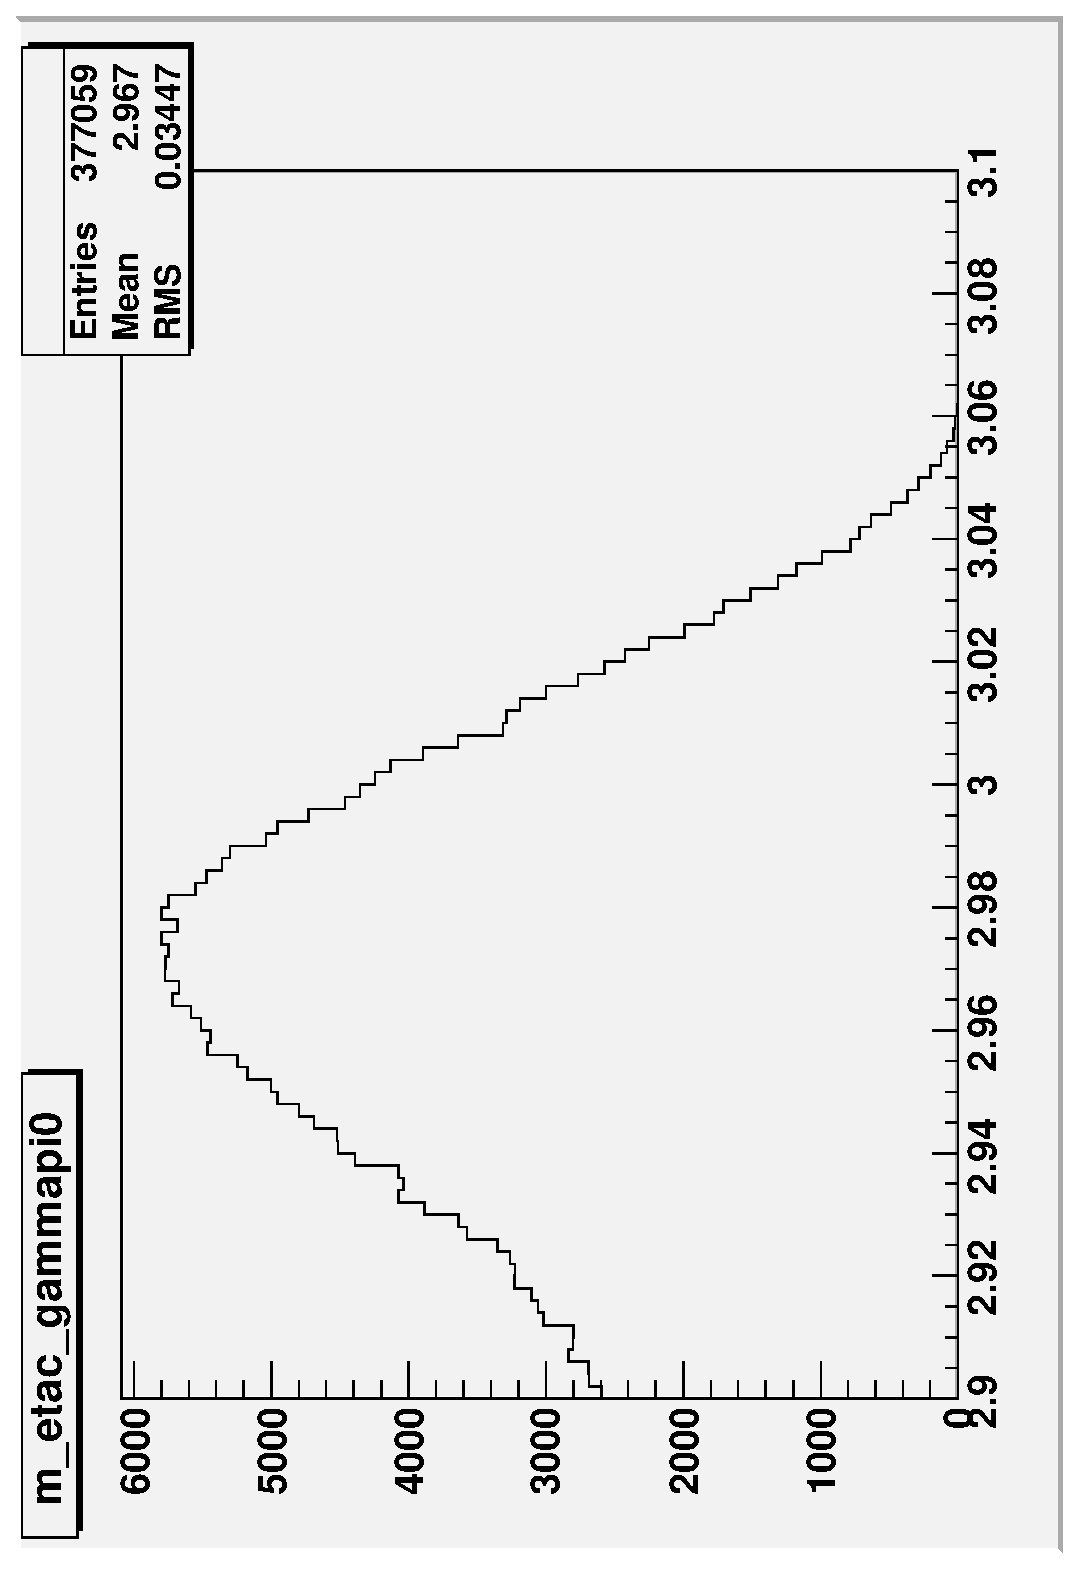
\includegraphics[width=0.5\textwidth,angle=270]{figure/12_m_etac_gammapi0.eps}
        \end{center}
        We can see that the signal of recoil of $\gamma$ and $\pi^0$ is \color{red}NOT \color{black}that obvious as expected.
        \end{frame}
%----------------------------------------------------------------------------------------

        \begin{frame}{Distribution of the recoil mass of $\pi^0$}
        \begin{center}
        \vskip -1.0cm
        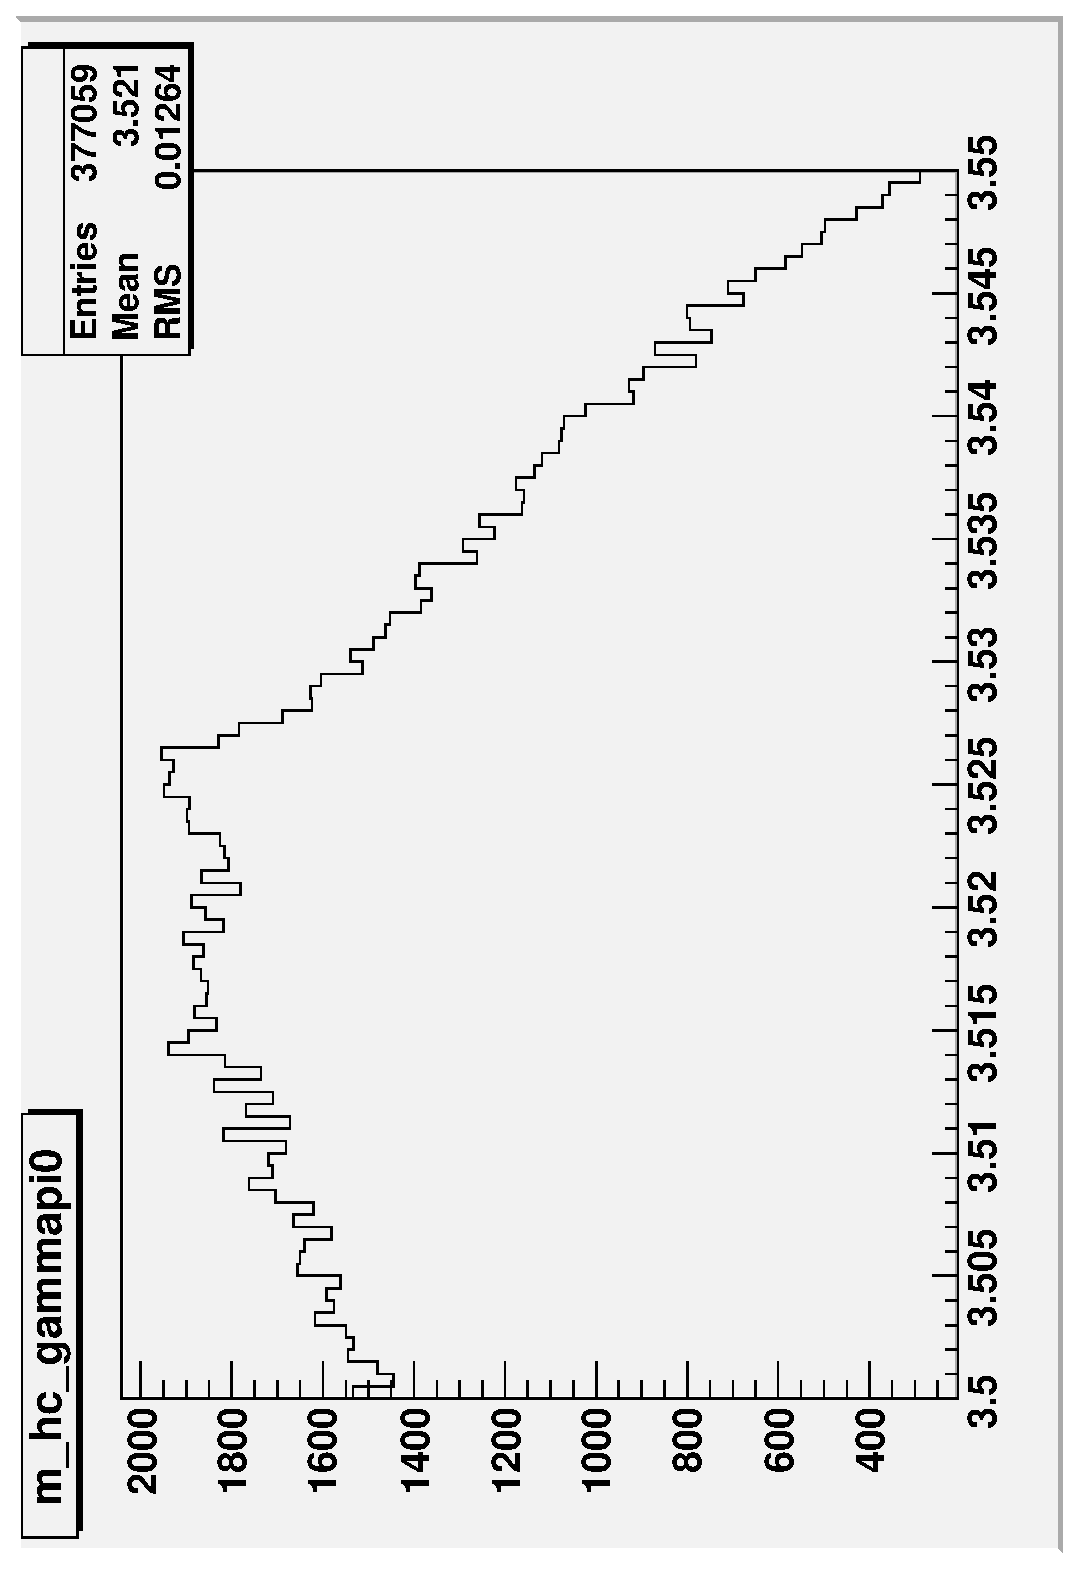
\includegraphics[width=0.5\textwidth,angle=270]{figure/12_m_hc_gammapi0.eps}
        \end{center}
        The signal corresponds with the results in the reference Measurement of $h_c(\sideset{^1}{_1}P)$ in $\psi'$ Decays(PRL 104, 132002(2010)).
        \end{frame}
%----------------------------------------------------------------------------------------
\end{document}
